% Official contribution: https://conferences.iaea.org/event/498/contributions/43613/
% Scheduled date: 2026-10-27.
\paragraph{Abstract}
\textit{Building an EXFOR~\cite{EXFOR} submission template and early community feedback}

This talk presents the development of a structured submission template to streamline experimental nuclear reaction data submission to EXFOR \url{https://exfor.io.oecd-nea.org/template/}. The approach addresses ambiguous metadata, inconsistent uncertainty descriptions, and missing experimental context that complicate compilation and reuse. Structured fields and defined uncertainty categories aim to preserve the scientific meaning of measurements while reducing manual interpretation. The template integrates into a collaborative GitLab workflow \url{https://git.oecd-nea.org/exfor} that supports traceable data submission, metadata review and validation before EXFOR compilation. A JSON Schema prototype, built on the NSC WPEC SG50~\cite{SG50-2023} framework, provides the basis for specifying the required information. Examples illustrate how the proposed format capture’s reaction details, bibliographic information, measured values, and associated uncertainties. A functional submission form and workflow prototype demonstrate progress towards direct contributions from experimentalists and automated processing. The presentation also discusses early community feedback gathered at WINS 2026 in Geel, Belgium~\cite{WINS2026}. This consultation explores information requirements, submission priorities, and preferences for the template’s structure. Further development will focus on modularisation, validation, and community testing, alongside agreement on mandatory fields and unresolved expert questions. The overall aim is to reduce compilation effort while keeping experimental knowledge complete, interpretable, and reusable.

\begin{figure}[htbp]
    \centering  
    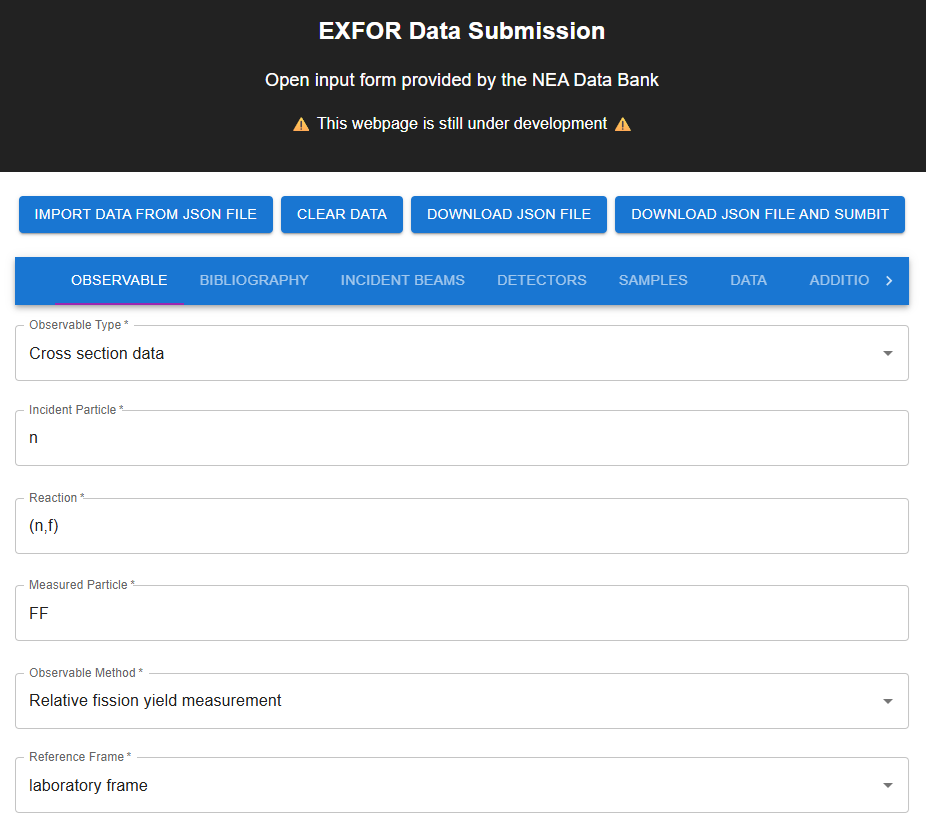
\includegraphics[width=0.8\textwidth]{figures/exfor_template_submission.png}
    \caption{Screenshot of the preliminary EXFOR Submission Form.}
    \label{fig:submission_form}
\end{figure}


\paragraph{Discussion}
% Source: Webex-Summary/day2.pdf; use the meeting date, not the filename.
Anastasia Georgiadou described a submission form backed by a schema and a GitLab workflow. Discussion covered mandatory metadata, copying tabulated values from existing tools, modular forms and reducing repeated entry. Participants raised the need to describe systematic uncertainties and correlations beyond simple per-point columns, together with reference standards and experimental context. Community feedback would inform further testing. A direct automated ingestion service was discussed as future work; the demonstrated workflow retained validation and human review before compilation.
